
\item A ball of mass \( m \) 0.5 kg is attached to the end of a string having length \( L \) 0.5 m. The ball is rotated on a horizontal circular path about vertical axis. The maximum tension that the string can bear is 324 N. The maximum possible value of angular velocity of ball (in radian/s) is
    \begin{center}
        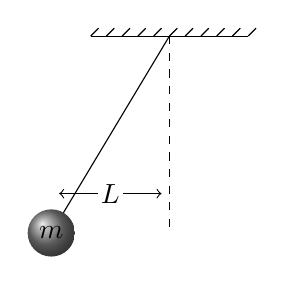
\begin{tikzpicture}
            % Drawing the ceiling
            \draw (-1, 0) -- (1, 0);
            \foreach \x in {-1,-0.8,...,1}
                \draw (\x, 0) -- (\x+0.1, 0.1);
            % Drawing the dashed line and string
            \draw[dashed] (0, 0) -- (0, -2.5);
            \draw (0, 0) -- (-1.5, -2.5);
            % Drawing the ball and label
            \shade[ball color=gray] (-1.5, -2.5) circle (0.3);
            \node at (-1.5, -2.5) {\( m \)};
            % Drawing the label L
            \draw[<->] (-0.1, -2) -- node[fill=white, inner sep=1pt] {\( L \)} (-1.4, -2);
        \end{tikzpicture}
    \end{center}
    \begin{tasks}(2)
        \task 9
        \task 18
        \task 27
        \task 36
    \end{tasks}
